
Hidden Markov Models (HMMs) are one of the most common sequence
probabilistic models, and have been applied to a wide variety of
tasks. HMMs are particular instances of directed probabilistic graphical models (or Bayesian networks) which have a chain topology. 
In a
Bayesian network, every random variable is represented as a node in a
graph, and the edges in the graph are directed and represent
probabilistic dependencies between the random variables. For an HMM, the random variables are divided into two sets, the 
\emph{observed variables}, $X = X_1\ldots X_N$, 
and the \emph{hidden variables} $Y = Y_1\ldots Y_N$.
In the HMM
terminology, the observed variables are called \emph{observations}, and the
hidden variables are called \emph{states}. 
The states are generated according to a first order Markov process, in which the $i^{th}$ state $Y_i$ depends only 
of the previous state $Y_{i-1}$. 
Two special states are the ${\tt start}$ symbol,
which starts the sequence, and 
the ${\tt stop}$ symbol, which ends the sequence. 
%Some textbooks describing HMMs omit the stop symbol. 
%While in some applications, one needs not to 
%consider It is useful to artificially introduce a special ``STOP'' state at the end of the sequence, which marks its end. This is useful for two reasons: it sibmplifies the notation, and it also allows our model to cope with sequences of any finite size (otherwise, how would our model cope with natural sentences, which can range from one or two words to dozens?).
%}
In addition, states emit observation symbols. In an HMM, it is assumed that all
observations are independent given the states
that generated them.


As you may find out with today's assignment, 
implementing the inference routines of the HMM can be challenging. We start with a small and very
simple (also very unrealistic!) example. The idea is that you may compute the desired
quantities by hand and check if your implementation yields the correct result. 

\begin{example}

Consider a person who is only interested in four activities: walking in the park ({\tt walk}), shopping ({\tt shop}), cleaning the apartment ({\tt clean}) and playing tennis ({\tt tennis}).
Also, consider that the choice of what the person does on a given day is determined exclusively by the weather on that day, which can be either {\tt rainy} or {\tt sunny}. 
Now, supposing that we observe what the person did on a sequence of days, the question is: 
can we use that information to predict the weather on each of those days? 
To tackle this problem, we assume 
that the weather behaves as a discrete Markov chain: the weather on a
given day depends only on 
the weather on the previous day. 
The entire system can be described as an HMM.

For example, assume we are asked to predict the weather conditions on two different
sequences of days. During these two sequences, we observed the person performing the following activities: 
\begin{itemize}
\item ``{\tt walk walk shop clean}'' 
\item ``{\tt clean walk tennis walk}''
\end{itemize}
This will be our test set.

Moreover, and in order to train our model, we are given access to three different sequences of days, containing both the activities performed by the person and the weather on those days, namely: 
\begin{itemize}
\item ``{\tt walk/rainy walk/sunny shop/sunny clean/sunny}'' 
\item ``{\tt walk/rainy walk/rainy shop/rainy clean/sunny}''
\item ``{\tt walk/sunny shop/sunny shop/sunny clean/sunny}''
\end{itemize}
This will be our training set.

%It is useful to artificially introduce a special ``STOP'' state at the end of the sequence, which marks its end. This is useful for two reasons: it simplifies the notation, and it also allows our model to cope with sequences of any finite size (otherwise, how would our model cope with natural sentences, which can range from one or two words to dozens?).

Figure \ref{hmm} shows the HMM model for the first sequence of the training set, which already includes the {\tt start} and 
{\tt stop} symbols. The notation is summarized in Table \ref{tab:hmm-simple-notation}.
\end{example}
 
\begin{figure}[ht]
\centering
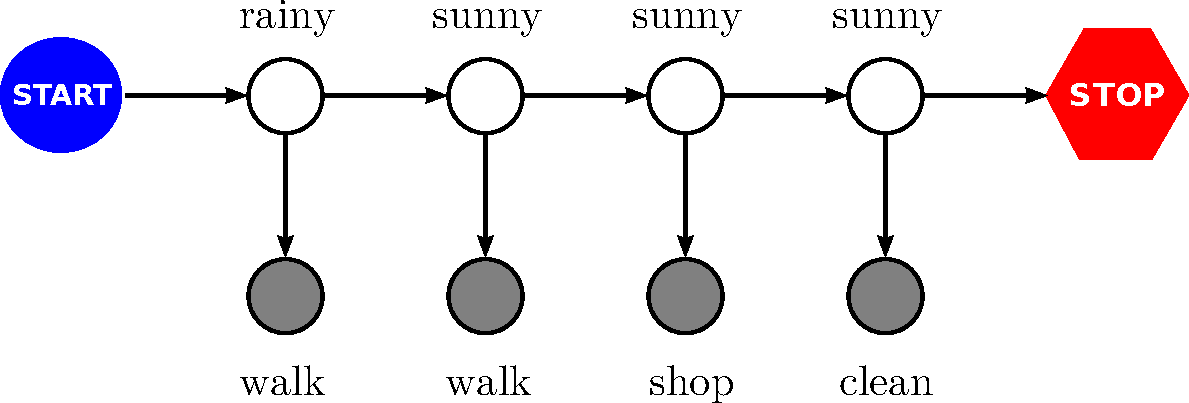
\includegraphics[width=0.7\textwidth]{figs/sequences/hmm_new}
\caption[HMM running example]{\label{fig:hmm}Diagram showing the conditional independence relations of the HMM. As an example, the variables are the values of the first sentence of the training set of the simple sequence.}
\end{figure}

\begin{table}[h]
\begin{center}
\begin{tabular}{|l|l|}
\hline
\multicolumn{2}{|c|}{HMM Notation}\\
\hline
\hline
$x$ & observed sequence ``{\tt walk walk shop clean}'' \\
\hline
$N = 4$ & observation length \\
\hline
$i$ & position in the sentence: $i \in \{1 \ldots N\}$ \\
\hline
$\vocab = \{\text{{\tt walk}},\text{{\tt shop}},\text{{\tt clean}},\text{{\tt tennis}}\}$ & observation set \\
\hline 
$j$ & index into the observation set $j \in \{1,\ldots, J\}$\\
\hline
$X_i = w_j$ & observation at position $i$ 
has value $w_j$\\
\hline 
$\statevocab = \{\text{{\tt rainy}},\text{{\tt sunny}}\}$ & state set\\
\hline 
$k$ & index into state set $k \in \{1,\ldots,K\}$\\
\hline
$Y_i = c_k$ & state at position $i$ has value $c_k$ \\ %acho que nao e necessario baralhar com os parenteses
\hline
\end{tabular}
\end{center}
\caption[HMM notation]{\label{tab:hmm-simple-notation} HMM notation for the simple example.}
\end{table}



\begin{exercise}
Load the simple sequence dataset. 
From the ipython command line create a simple sequence object and look
at the training and test set.
\begin{python}
import lxmls.readers.simple_sequence as ssr
simple = ssr.SimpleSequence()
print(simple.train)

[walk/rainy walk/sunny shop/sunny clean/sunny , walk/rainy walk/rainy shop/rainy clean/sunny , walk/sunny shop/sunny shop/sunny clean/sunny ]

print(simple.test)

[walk/rainy walk/sunny shop/sunny clean/sunny , clean/sunny walk/sunny tennis/sunny walk/sunny ]
\end{python}
Get in touch with the classes used to store the sequences, you will need this for the next exercise. Note that each label is internally stored as a number. This number can be used as index of an array to store information regarding that label.
\begin{python}
for sequence in simple.train.seq_list:
    print(sequence)

walk/rainy walk/sunny shop/sunny clean/sunny
walk/rainy walk/rainy shop/rainy clean/sunny
walk/sunny shop/sunny shop/sunny clean/sunny

for sequence in simple.train.seq_list:
    print(sequence.x)

[0, 0, 1, 2]
[0, 0, 1, 2]
[0, 1, 1, 2]

for sequence in simple.train.seq_list:
    print(sequence.y)

[0, 1, 1, 1]
[0, 0, 0, 1]
[1, 1, 1, 1]
\end{python}

\end{exercise}

The probability distributions $P(Y_{i}|Y_{i-1})$ are called \emph{transition probabilities}; the distributions 
$P(Y_{1}|Y_{0} = {\tt start})$ are the \emph{initial probabilities}, and 
$P(Y_{N+1}={\tt stop} |Y_{N})$ the \emph{final probabilities}.%
\footnote{Note that the initial and final probabilities 
are asymmetric.} %
Finally, the distributions $P(X_i|Y_i)$ are called \emph{emission probabilities}. 


A first order HMM model has the following independence assumptions over the joint distribution $P(X=x,Y=y)$:
\begin{itemize}
  \item \textbf{Independence of previous states.} The probability of
    being in a given state at position $i$ only depends on
    the state of the previous position $i-1$. Formally, 
    \begin{equation*}
    P (Y_i = y_i | Y_{i-1} = y_{i-1}, Y_{i-2} = y_{i-2}, \ldots, Y_1 = y_1) = P (Y_i = y_i | Y_{i-1} = y_{i-1})
    \end{equation*} 
    defining a first order Markov chain.%
    \footnote{The order of the Markov chain depends on the number of previous positions taken into account. 
    The remainder of the exposition can be easily extended to higher order HMMs, giving the model more generality, 
    but making inference more expensive.}
  \item \textbf{Homogeneous transition.} The probability of
    making a transition from state $c_l$ to state $c_k$ is independent of
    the particular position in the sequence. That is, for all $i,t \in \{1,\ldots,N\}$,
     \begin{equation*}
    P (Y_i = c_k | Y_{i-1} = c_l) =  P (Y_{t} = c_k | Y_{t-1} = c_l)
     \end{equation*}
    % , so we can simply write //novamente, P_{\mathrm{trans}} so e introduzido depois
     %\begin{equation*}
    %P (Y_i = c_k | Y_{i-1} = c_l) = P_{\mathrm{trans}}(c_k|c_l)
     %\end{equation*}
  \item \textbf{Observation independence.}  The probability of
    observing $X_i = x_i$ at position $i$ is fully determined by the state $Y_i$
    at that position. Formally, 
     \begin{equation*}
     P (X_i = x_i | Y_1=y_1, \ldots, Y_i=y_i, \ldots, Y_N=y_N) = P(X_i = x_i | Y_i = y_i)
      \end{equation*}
      This probability is independent of the
    particular position so, for every $i$ and $t$, we can write:  
     \begin{equation*}
    P(X_i = w_j | Y_i = c_k) = P(X_{t} = w_j | Y_{t} = c_k)
     \end{equation*}
    % = P_{\mathrm{emiss}}(w_j|c_k)$.
\end{itemize}
These conditional independence assumptions are crucial to allow
efficient inference, as it will be described.

%ESTA DEFINIDO LA EM CIMA: We also need to define \emph{initial probabilities}, the probability of starting 
% at each state, and  \emph{final probabilities}, the probability of ending the sequence given that we are at a particular state.
%Furthermore, when dealing with text, it is usual to break the homogeneous transition for the last position, and model the final transitions as independent parameters.

 The distributions that define the HMM model are summarized in Table
\ref{tab:hmm-dist}. 
For each one
of them we will use a short notation to simplify the exposition.
\begin{table}[h]
\begin{center}
\begin{tabular}{|l|l|l|l|}
\hline
\multicolumn{4}{|c|}{HMM distributions}\\
\hline
Name & probability distribution & short notation & array size\\
\hline
\textbf{initial probability} & $P(Y_1 = c_k | Y_0 = \text{\tt start})$ & $P_{\mathrm{init}}(c_k|\text{\tt start})$ & $K$ \\
\hline
\textbf{transition probability} & $P(Y_{i}=c_k|Y_{i-1} = c_l)$ & $P_{\mathrm{trans}}(c_k|c_l)$ & $K\times K$\\
\hline
\textbf{final probability} & $P(Y_{N+1} = \text{\tt stop} | Y_N = c_k)$ & $P_{\mathrm{final}}(\text{\tt stop}|c_k)$ & $K$\\
\hline
\textbf{emission probability} & $P(X_i=w_j| Y_i = c_k)$ & $P_{\mathrm{emiss}}(w_j|c_k)$ & $J \times K$ \\
\hline
\end{tabular}
\end{center}
\caption[HMM probability distributions]{\label{tab:hmm-dist} HMM probability distributions.}
\end{table}

The joint distribution can be expressed as:
\begin{eqnarray}\label{eqn:hmm}
\lefteqn{P(X_1=x_1,\ldots,X_N=x_N,Y_1=y_1,\ldots,Y_N=y_N)=}\nonumber\\
&&
P_{\mathrm{init}}(y_1|\text{\tt start}) 
\times
\left(
\prod_{i=1}^{N-1} P_{\mathrm{trans}}(y_{i+1}|y_i)
\right)
\times
P_{\mathrm{final}}(\text{\tt stop}|y_N)
\times 
\prod_{i=1}^{N} P_{\mathrm{emiss}}(x_i|y_i),
\end{eqnarray}
which for the example of Figure \ref{fig:hmm} is:
\begin{eqnarray}  \label{eqn:hmm_ex}
\lefteqn{P(X_1=x_1,\ldots,X_4=x_4,Y_1=y_1,\ldots,Y_4=y_4)=}\nonumber\\
&&
P_{\mathrm{init}}(\text{\tt rainy}|\text{\tt start}) 
\times
P_{\mathrm{trans}}(\text{\tt sunny}|\text{\tt rainy}) 
\times
P_{\mathrm{trans}}(\text{\tt sunny}|\text{\tt sunny}) 
\times
P_{\mathrm{trans}}(\text{\tt sunny}|\text{\tt sunny}) 
\times\nonumber\\&&
P_{\mathrm{final}}(\text{\tt stop}|\text{\tt sunny}) 
\times
P_{\mathrm{emiss}}(\text{\tt walk}|\text{\tt rainy}) 
\times
P_{\mathrm{emiss}}(\text{\tt walk}|\text{\tt sunny}) 
\times
P_{\mathrm{emiss}}(\text{\tt shop}|\text{\tt sunny}) \nonumber\\&&
\times
P_{\mathrm{emiss}}(\text{\tt clean}|\text{\tt sunny}).
\end{eqnarray}

In the next section we turn our attention to estimating the different
probability distributions of the model.
